%%%%%%%%%%%%%%%%%%%%%%%%%%%%%%%%%%%%%%%%%
% Beamer Presentation
% LaTeX Template
% Version 2.0 (March 8, 2022)
%
% This template originates from:
% https://www.LaTeXTemplates.com
%
% Author:
% Vel (vel@latextemplates.com)
%
% License:
% CC BY-NC-SA 4.0 (https://creativecommons.org/licenses/by-nc-sa/4.0/)
%
%%%%%%%%%%%%%%%%%%%%%%%%%%%%%%%%%%%%%%%%%

%----------------------------------------------------------------------------------------
%	PACKAGES AND OTHER DOCUMENT CONFIGURATIONS
%----------------------------------------------------------------------------------------

\documentclass[
	11pt, % Set the default font size, options include: 8pt, 9pt, 10pt, 11pt, 12pt, 14pt, 17pt, 20pt
	%t, % Uncomment to vertically align all slide content to the top of the slide, rather than the default centered
	%aspectratio=169, % Uncomment to set the aspect ratio to a 16:9 ratio which matches the aspect ratio of 1080p and 4K screens and projectors
]{beamer}

\graphicspath{{Images/}{./}} % Specifies where to look for included images (trailing slash required)

\usepackage{booktabs} % Allows the use of \toprule, \midrule and \bottomrule for better rules in tables

%----------------------------------------------------------------------------------------
%	SELECT LAYOUT THEME
%----------------------------------------------------------------------------------------

% Beamer comes with a number of default layout themes which change the colors and layouts of slides. Below is a list of all themes available, uncomment each in turn to see what they look like.

%\usetheme{default}
%\usetheme{AnnArbor}
%\usetheme{Antibes}
%\usetheme{Bergen}
%\usetheme{Berkeley}
%\usetheme{Berlin}
\usetheme{Boadilla} %me gusta
%\usetheme{CambridgeUS}
%\usetheme{Copenhagen}
%\usetheme{Darmstadt}
%\usetheme{Dresden}
%\usetheme{Frankfurt}
%\usetheme{Goettingen} %dos dos
%\usetheme{Hannover} %dos dos
%\usetheme{Ilmenau}
%\usetheme{JuanLesPins}
%\usetheme{Luebeck}
%\usetheme{Madrid}
%\usetheme{Malmoe}
%\usetheme{Marburg}
%\usetheme{Montpellier}
%\usetheme{PaloAlto}
%\usetheme{Pittsburgh}
%\usetheme{Rochester} %muy flat
%\usetheme{Singapore}
%\usetheme{Szeged}
%\usetheme{Warsaw}

%----------------------------------------------------------------------------------------
%	SELECT COLOR THEME
%----------------------------------------------------------------------------------------

% Beamer comes with a number of color themes that can be applied to any layout theme to change its colors. Uncomment each of these in turn to see how they change the colors of your selected layout theme.

%\usecolortheme{albatross}
%\usecolortheme{beaver}
%\usecolortheme{beetle}
%\usecolortheme{crane}
%\usecolortheme{dolphin}
%\usecolortheme{dove}
%\usecolortheme{fly}
%\usecolortheme{lily} %default
%\usecolortheme{monarca}
%\usecolortheme{seagull}
%\usecolortheme{seahorse}
%\usecolortheme{spruce}
%\usecolortheme{whale}
%\usecolortheme{wolverine}

%----------------------------------------------------------------------------------------
%	SELECT FONT THEME & FONTS
%----------------------------------------------------------------------------------------

% Beamer comes with several font themes to easily change the fonts used in various parts of the presentation. Review the comments beside each one to decide if you would like to use it. Note that additional options can be specified for several of these font themes, consult the beamer documentation for more information.

\usefonttheme{default} % Typeset using the default sans serif font
%\usefonttheme{serif} % Typeset using the default serif font (make sure a sans font isn't being set as the default font if you use this option!)
%\usefonttheme{structurebold} % Typeset important structure text (titles, headlines, footlines, sidebar, etc) in bold
%\usefonttheme{structureitalicserif} % Typeset important structure text (titles, headlines, footlines, sidebar, etc) in italic serif
%\usefonttheme{structuresmallcapsserif} % Typeset important structure text (titles, headlines, footlines, sidebar, etc) in small caps serif

%------------------------------------------------

%\usepackage{mathptmx} % Use the Times font for serif text
\usepackage{palatino} % Use the Palatino font for serif text

%\usepackage{helvet} % Use the Helvetica font for sans serif text
\usepackage[default]{opensans} % Use the Open Sans font for sans serif text
%\usepackage[default]{FiraSans} % Use the Fira Sans font for sans serif text
%\usepackage[default]{lato} % Use the Lato font for sans serif text

%----------------------------------------------------------------------------------------
%	SELECT INNER THEME
%----------------------------------------------------------------------------------------

% Inner themes change the styling of internal slide elements, for example: bullet points, blocks, bibliography entries, title pages, theorems, etc. Uncomment each theme in turn to see what changes it makes to your presentation.

%\useinnertheme{default}
\useinnertheme{circles}
%\useinnertheme{rectangles}
%\useinnertheme{rounded}
%\useinnertheme{inmargin}

%----------------------------------------------------------------------------------------
%	SELECT OUTER THEME
%----------------------------------------------------------------------------------------

% Outer themes change the overall layout of slides, such as: header and footer lines, sidebars and slide titles. Uncomment each theme in turn to see what changes it makes to your presentation.

%\useoutertheme{default}
%\useoutertheme{infolines}
%\useoutertheme{miniframes}
%\useoutertheme{smoothbars}
%\useoutertheme{sidebar}
%\useoutertheme{split}
%\useoutertheme{shadow}
%\useoutertheme{tree}
%\useoutertheme{smoothtree}

%\setbeamertemplate{footline} % Uncomment this line to remove the footer line in all slides
%\setbeamertemplate{footline}[page number] % Uncomment this line to replace the footer line in all slides with a simple slide count

%\setbeamertemplate{navigation symbols}{} % Uncomment this line to remove the navigation symbols from the bottom of all slides

%----------------------------------------------------------------------------------------
%	PRESENTATION INFORMATION
%----------------------------------------------------------------------------------------

\title[REDES NEURONALES]{Aprendizaje por refuerzo y no supervisado en redes neuronales} % The short title in the optional parameter appears at the bottom of every slide, the full title in the main parameter is only on the title page

%\subtitle{Optional Subtitle} % Presentation subtitle, remove this command if a subtitle isn't required

\author[Luis Ballado]{Luis Ballado} % Presenter name(s), the optional parameter can contain a shortened version to appear on the bottom of every slide, while the main parameter will appear on the title slide

\institute[CINVESTAV]{CINVESTAV - UNIDAD TAMAULIPAS \\ \smallskip \textit{luis.ballado@cinvestav.mx}} % Your institution, the optional parameter can be used for the institution shorthand and will appear on the bottom of every slide after author names, while the required parameter is used on the title slide and can include your email address or additional information on separate lines

\date[\today]{\today} % Presentation date or conference/meeting name, the optional parameter can contain a shortened version to appear on the bottom of every slide, while the required parameter value is output to the title slide

%----------------------------------------------------------------------------------------

\begin{document}

%----------------------------------------------------------------------------------------
%	TITLE SLIDE
%----------------------------------------------------------------------------------------

\begin{frame}
	\titlepage % Output the title slide, automatically created using the text entered in the PRESENTATION INFORMATION block above
\end{frame}

%----------------------------------------------------------------------------------------
%	TABLE OF CONTENTS SLIDE
%----------------------------------------------------------------------------------------

% The table of contents outputs the sections and subsections that appear in your presentation, specified with the standard \section and \subsection commands. You may either display all sections and subsections on one slide with \tableofcontents, or display each section at a time on subsequent slides with \tableofcontents[pausesections]. The latter is useful if you want to step through each section and mention what you will discuss.

\begin{frame}
	\frametitle{Contenido} % Slide title, remove this command for no title
	
	\tableofcontents % Output the table of contents (all sections on one slide)
	%\tableofcontents[pausesections] % Output the table of contents (break sections up across separate slides)
\end{frame}

%----------------------------------------------------------------------------------------
%	PRESENTATION BODY SLIDES
%----------------------------------------------------------------------------------------

\section{Introducción} % Sections are added in order to organize your presentation into discrete blocks, all sections and subsections are automatically output to the table of contents as an overview of the talk but NOT output in the presentation as separate slides

%------------------------------------------------

\begin{frame}
  \frametitle{Introducción}

  Desde la primera mitad del siglo XX se han desarrollado modelos computacionales que han intentado emular el comportamiento del cerebro humano. Aunque se han propuesto una gran cantidad de ellos, todos usan una estructura en red en la cual los nodos o neuronas son procesos numéricos que involucran estados de otros nodos según sus uniones. Una clase de estos modelos computacionales son las Redes de Neuronas Arificiales.

  \bigskip % Vertical whitespace
  
  Por su marcada habilidad para obtener resultados de datos complicados e imprecisos, pueden utilizarse para extraer patrones y detectar tramas que son muy difíciles de apreciar por humanos u otras técnicas computacionales.
  
\end{frame}

\begin{frame}
  \frametitle{Esquema básico del trabajo con RNA}
  
  \begin{figure}
    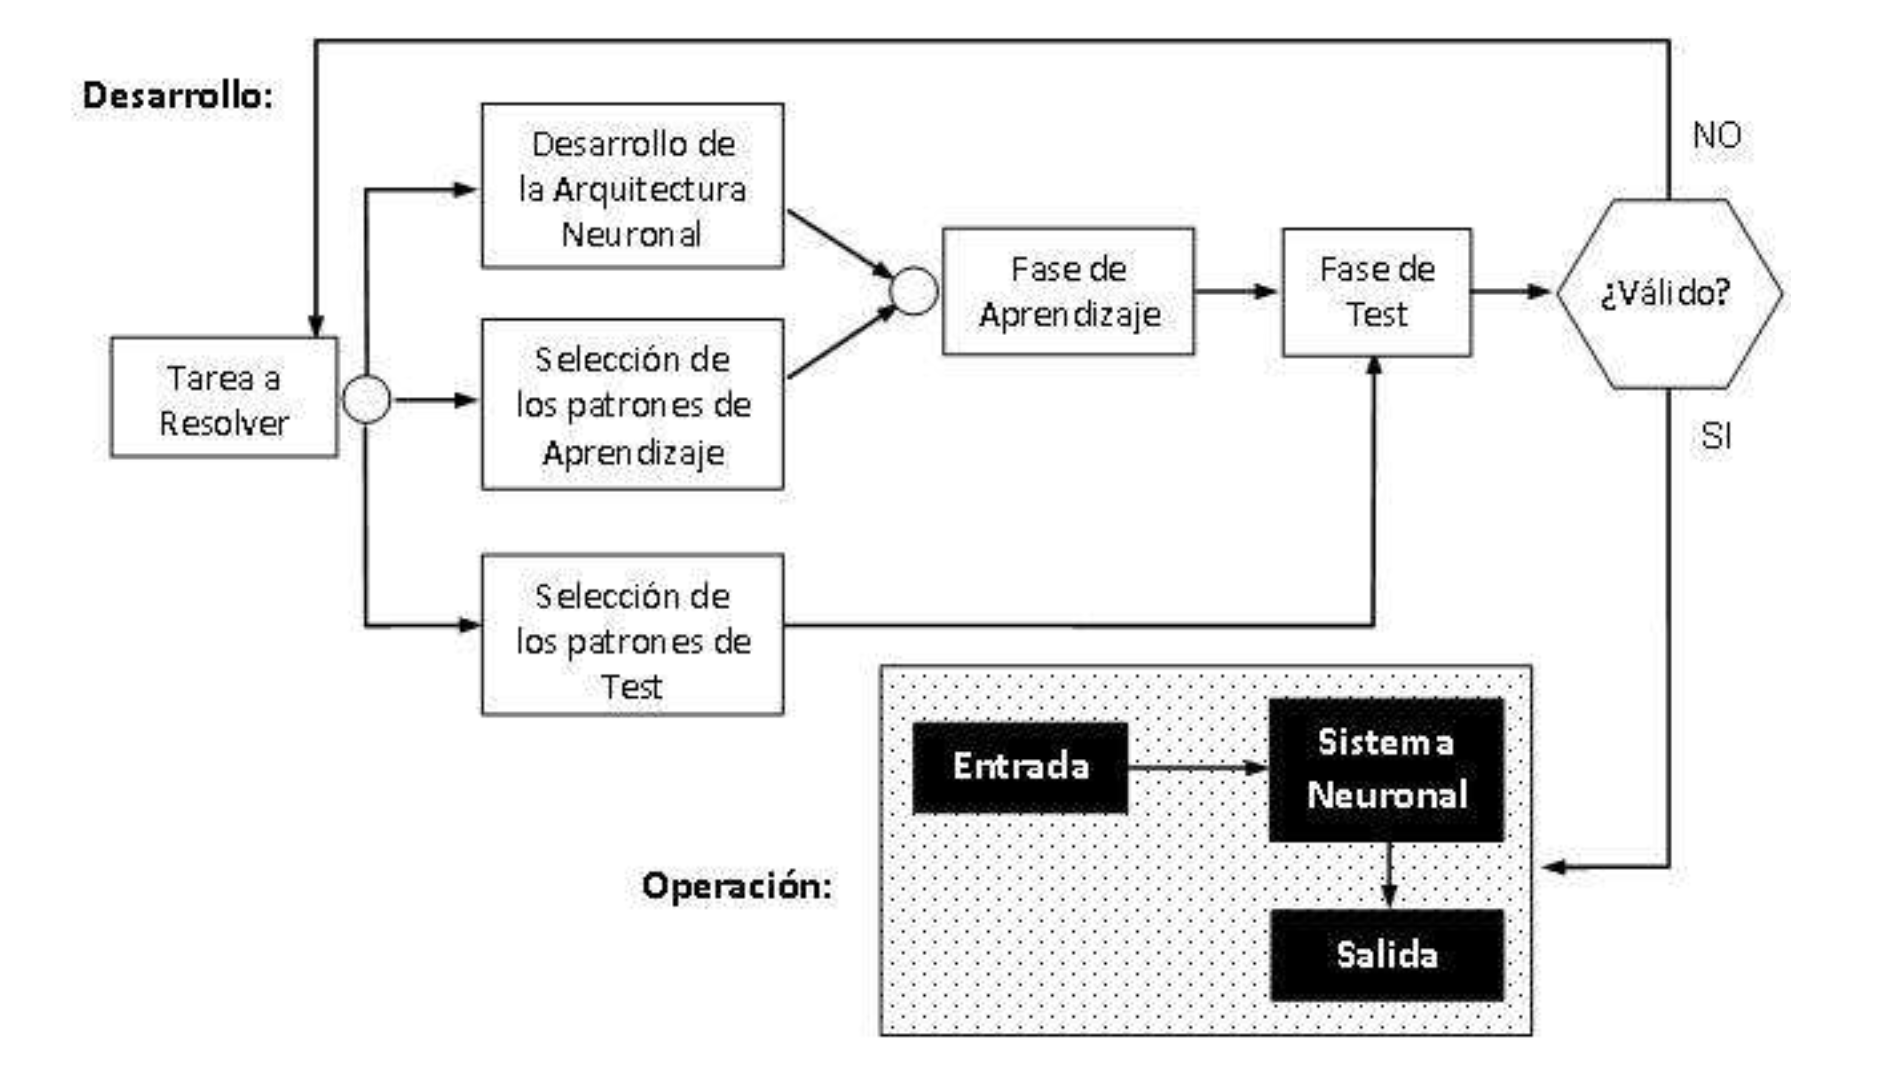
\includegraphics[width=0.8\linewidth]{rna_.png}
  \end{figure}
\end{frame}

\begin{frame}
  
  % Quote example
  \begin{quote}
    Las redes neuronales son conjunto de elementos de cálculo simples, usualmente adaptativos, interconectados masivamente en paralelo y con una organización jerárquica que le permite interactuar con algún sistema del mismo modo que lo hace el sistema nervioso biológico.\\
    \bigskip % Vertical whitespace
    --- T. Kohonen. Self-organization and associative memory. Springer Verlag, New York, 1989.\ldots
  \end{quote}
  
  \bigskip % Vertical whitespace
    
\end{frame}


\begin{frame}
  \frametitle{El inicio - la neurona artificial}

  Entre las décadas de 1950 y 1960 el científico Frank Rosenblatt, inspirado en el trabajo de Warren McCulloch y Walter Pitts creó el \alert{Perceptron}, la unidad desde donde nacería y se potenciarían las redes neuronales artificiales.

  \bigskip % Vertical whitespace

  Un perceptron toma varias entradas binarias x1, x2, etc. para producir una sóla salida binaria. Para calcular la salida, Rosenblatt introduce el concepto de "pesos" w1, w2, etc. que es un número real que expresa la importancia de la respectiva entrada con la respectiva salida. La salida de la neurona será 1 ó 0 si la suma de la multiplicación de pesos por entradas es mayor o menor a un determinado umbral.\\
  \bigskip % Vertical whitespace
  Sus principales usos son decisiones binarias sencillas como compuertas lógicas
\end{frame}

\begin{frame}
  
  \begin{figure}
    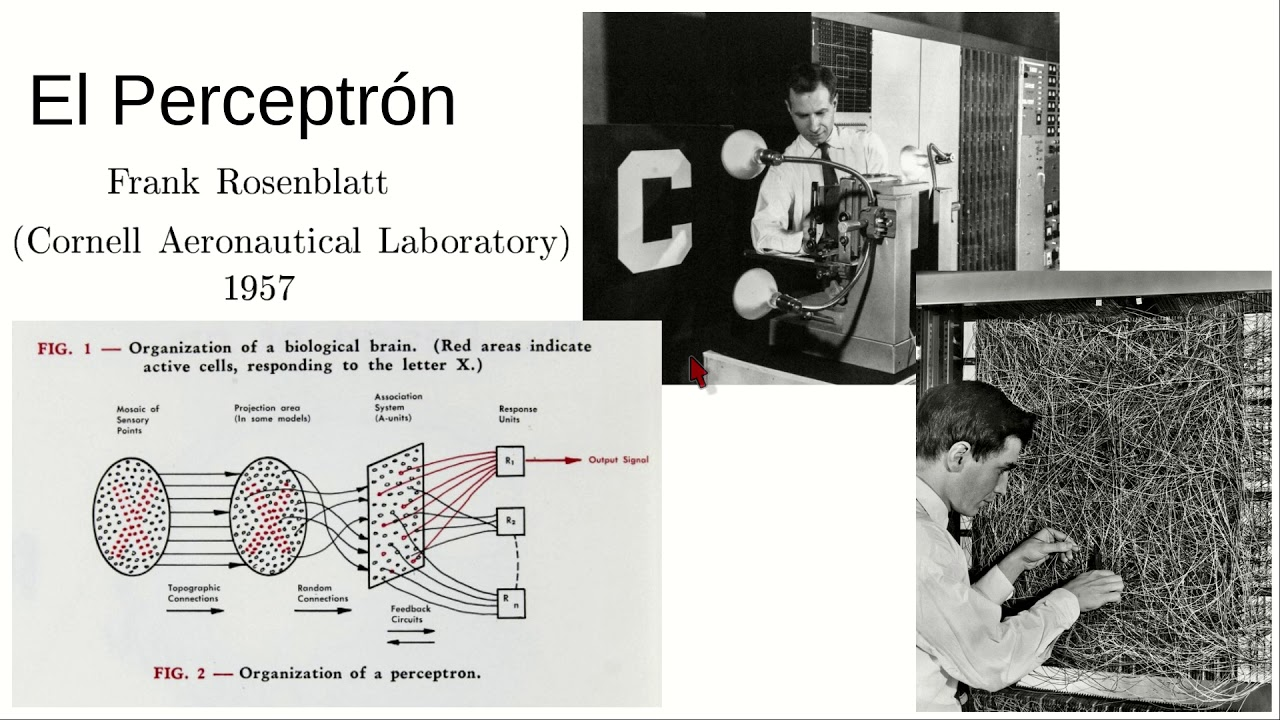
\includegraphics[width=0.8\linewidth]{percep.jpg}
  \end{figure}
\end{frame}

\begin{frame}
  
  \begin{figure}
    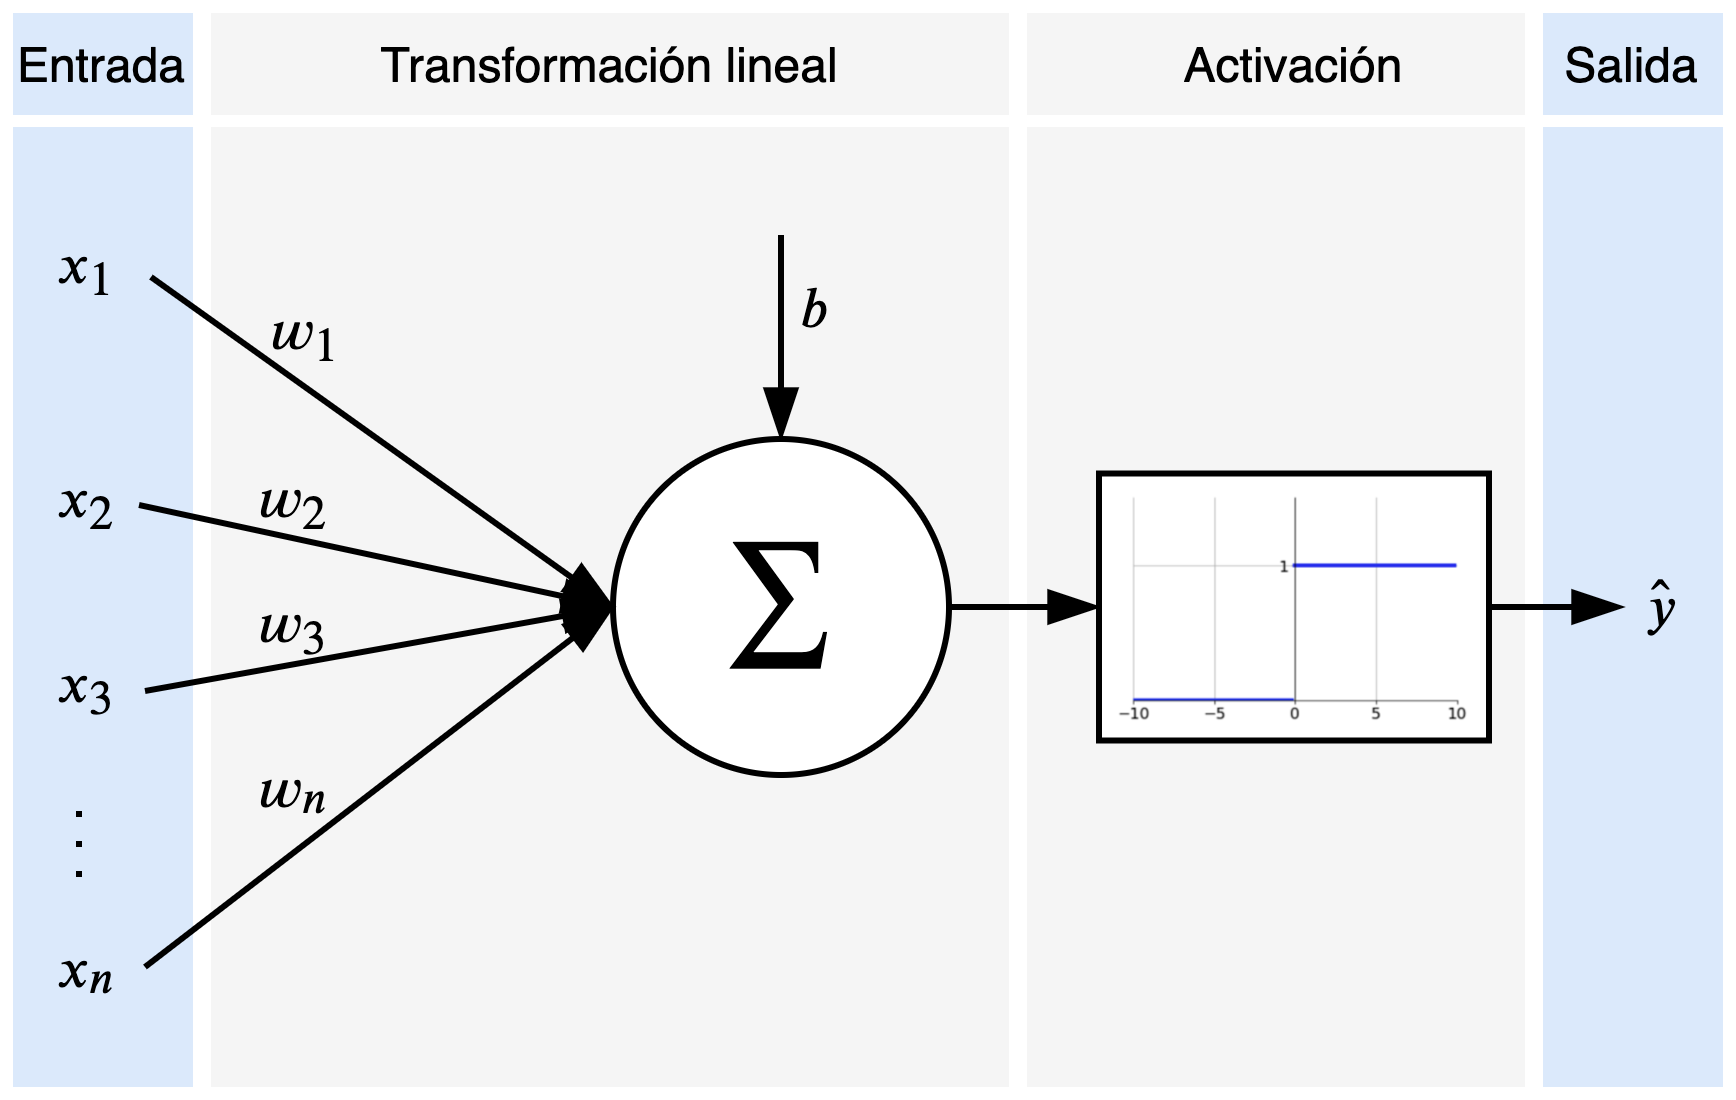
\includegraphics[width=0.8\linewidth]{perceptron.png}
  \end{figure}
\end{frame}

\begin{frame}
  \frametitle{Multilayer Perceptron - 1965}

  Es solo una ampliación del modelo que se conoce del perceptron de una sola neurona a más de una. Apareciendo el concepto de capas de entrada, oculta y salida. Pero los valores de entrada/salida binarios.

  \bigskip % Vertical whitespace

  Los valores de los pesos eran asignados manualmente - Entre más perceptrones en las capas, mucho más difícil conseguir los pesos para obtener salidas deseadas.
  
\end{frame}

\begin{frame}
  
  \begin{figure}
    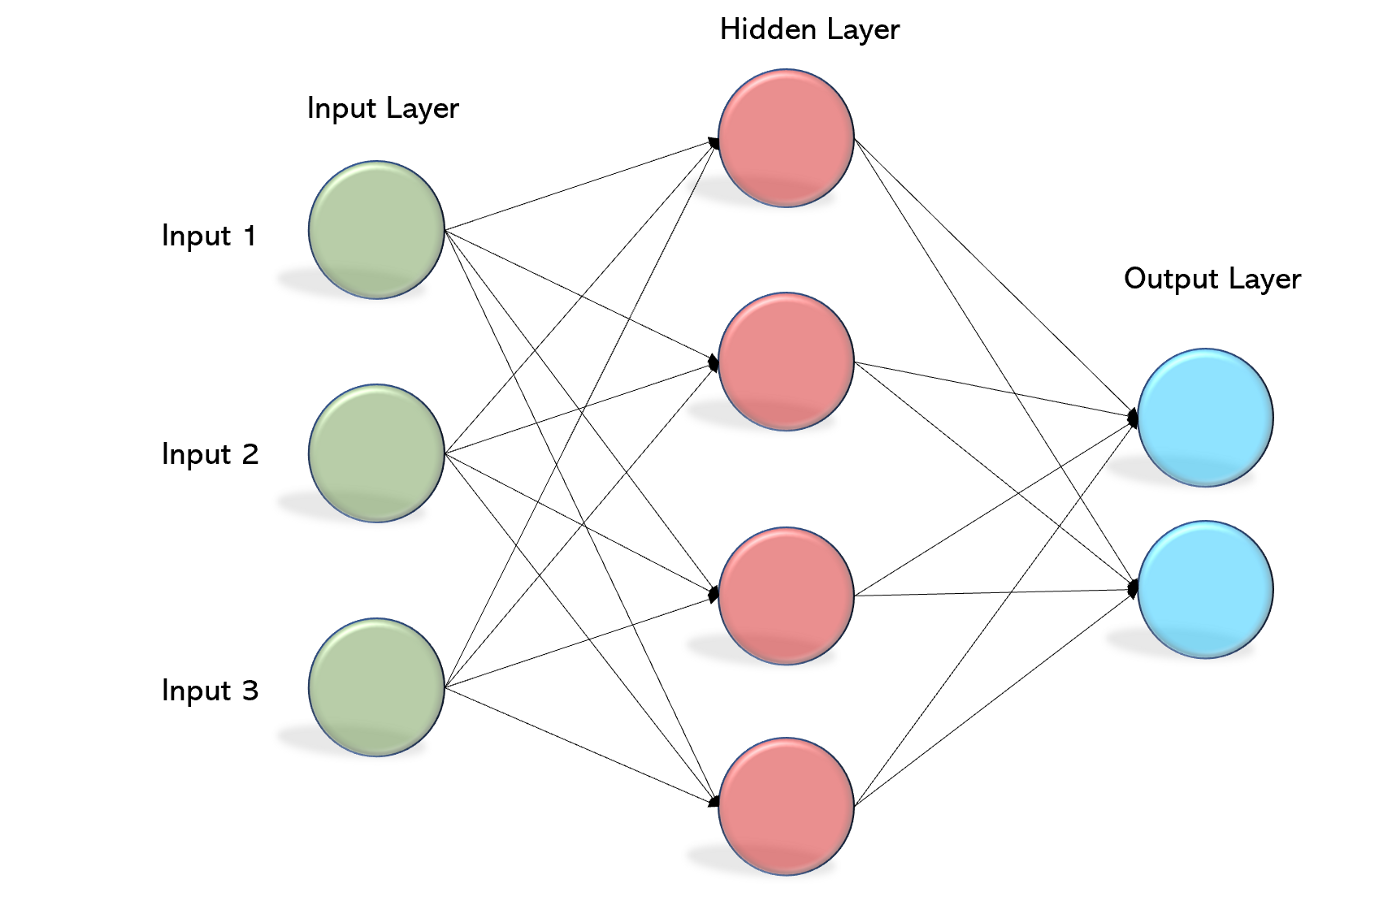
\includegraphics[width=0.8\linewidth]{m_perceptron.png}
  \end{figure}
\end{frame}

\begin{frame}
  \frametitle{Neuronas Sigmoides - 1980's}

  Para poder lograr que las redes de neuronas aprendan solas fue necesario introducir un nuevo tipo de neuronas llamadas \alert{Sigmoides} que son similares al perceptron, pero estas permiten que las entradas puedan tomar valores reales

  \bigskip % Vertical whitespace

  La función sigmoide definida como $d(z) = \frac{1}{1+e^{-z}}$ es la primer función de activación

  \begin{figure}
    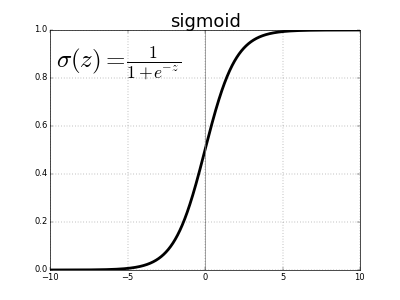
\includegraphics[width=0.5\linewidth]{sigmoid.png}
  \end{figure}
  
\end{frame}

\begin{frame}
  \frametitle{Backpropagation - 1986}

  Gracias al algoritmo de backpropagation se hizo posible entrenar redes neuronales de multiples capas de manera supervisada. Al calcular el error obtenido en la entrada e ir propagando hacia las capas anteriores. Se hacen ajustes pequeños (minimizando el costo) en cada iteración para lograr que la red aprenda consiguiendo que la red pueda clasificar las entradas correctamente.
  
  
\end{frame}

\begin{frame}
  \frametitle{Convolutional Neural Network - 1989}

  Son redes multicapa que toman su inspiración del cortex visual de los animales. Es útil en varias aplicaciones, principalmente \alert{procesamiento de imágenes}. La primera CNN fué propuesta por Yann LeCun y estaba enfocada en el reconocimiento de letras manuscritas MNIST http://yann.lecun.com/exdb/mnist/ 
  
  \bigskip % Vertical whitespace

  La arquitectura constaba de varias capas que implementaban la extracción de características y luego clasificar.\\
  La imágen se divide en campos receptivos que alimentan una capa convolucional que extrae caracteristicas de la imágen de entrada. (por ejemplo, detectar lineas verticales, vértices, etc.)
  
\end{frame}

\begin{frame}
  \frametitle{Long Short Term Memory / Recurrent Neural Network - 1997}

  Esta arquitectura permite conexiones "hacia atrás" entre las capas. Esto las hace buenas para procesar datos de tipo historicos.
  
  \bigskip % Vertical whitespace

  Consisten en unas celdas de memoria que permiten a la red recordar valores por períodos cortos o largos.\\
  Sus aplicaciones se pueden ver en el reconocimiento de voz, de escritura, text to speech por mencionar algunas
\end{frame}

\begin{frame}
  \frametitle{Deep Belief Networks - 2006}

  Demostraron que utilizar pesos aleatorios al inicializar las redes son una mala idea: por ejemplo al utilizar backpropagation con descenso por gradiente muchas veces se caía en mínimos locales, sin lograr optimizar los pesos. Lo mejor es utilizar una asignación de pesos inteligente mediante un preentrenamiento de las capas de la red "pre-entrenamiento"
  
  \bigskip % Vertical whitespace

  Se cree que ese preentrenamiento es una de las causas de la gran mejora en las redes neuronales y permitir el deep learning
  
\end{frame}

\begin{frame}
  \frametitle{Generative Adversarial Networks - 2014}

  La idea detrás es de tener dos modelos de redes neuronales compitiendo.
  
  \bigskip % Vertical whitespace

  Uno llamado Generador, toma inicialmente "datos basura" como entrada y genera muestras.\\
  El otro modelo, llamado Discriminador que recibe a la vez muestras del Generador y del conjunto de entrenamiento y deberá ser capaz de diferenciar entre las dos fuentes.

  \bigskip % Vertical whitespace

  Sus aplicaciones principales son la generación de imágenes realistas, pero también la mejora de imágenes ya existentes, o generar textos en imágenes o hasta el desarrollo de moléculas para industria farmacéutica.
  
\end{frame}


%------------------------------------------------
\section{Paradigmas de Aprendizaje}
\begin{frame}
  \frametitle{Paradigmas de Aprendizaje}
  Mecanismos que permiten que podamos procesar toda aquella información nueva que percibimos para acabar transformándola en conocimiento. La mayoria de los algoritmos dentro del ML se pueden clasificar en estos tres grupos.

  \begin{figure}
    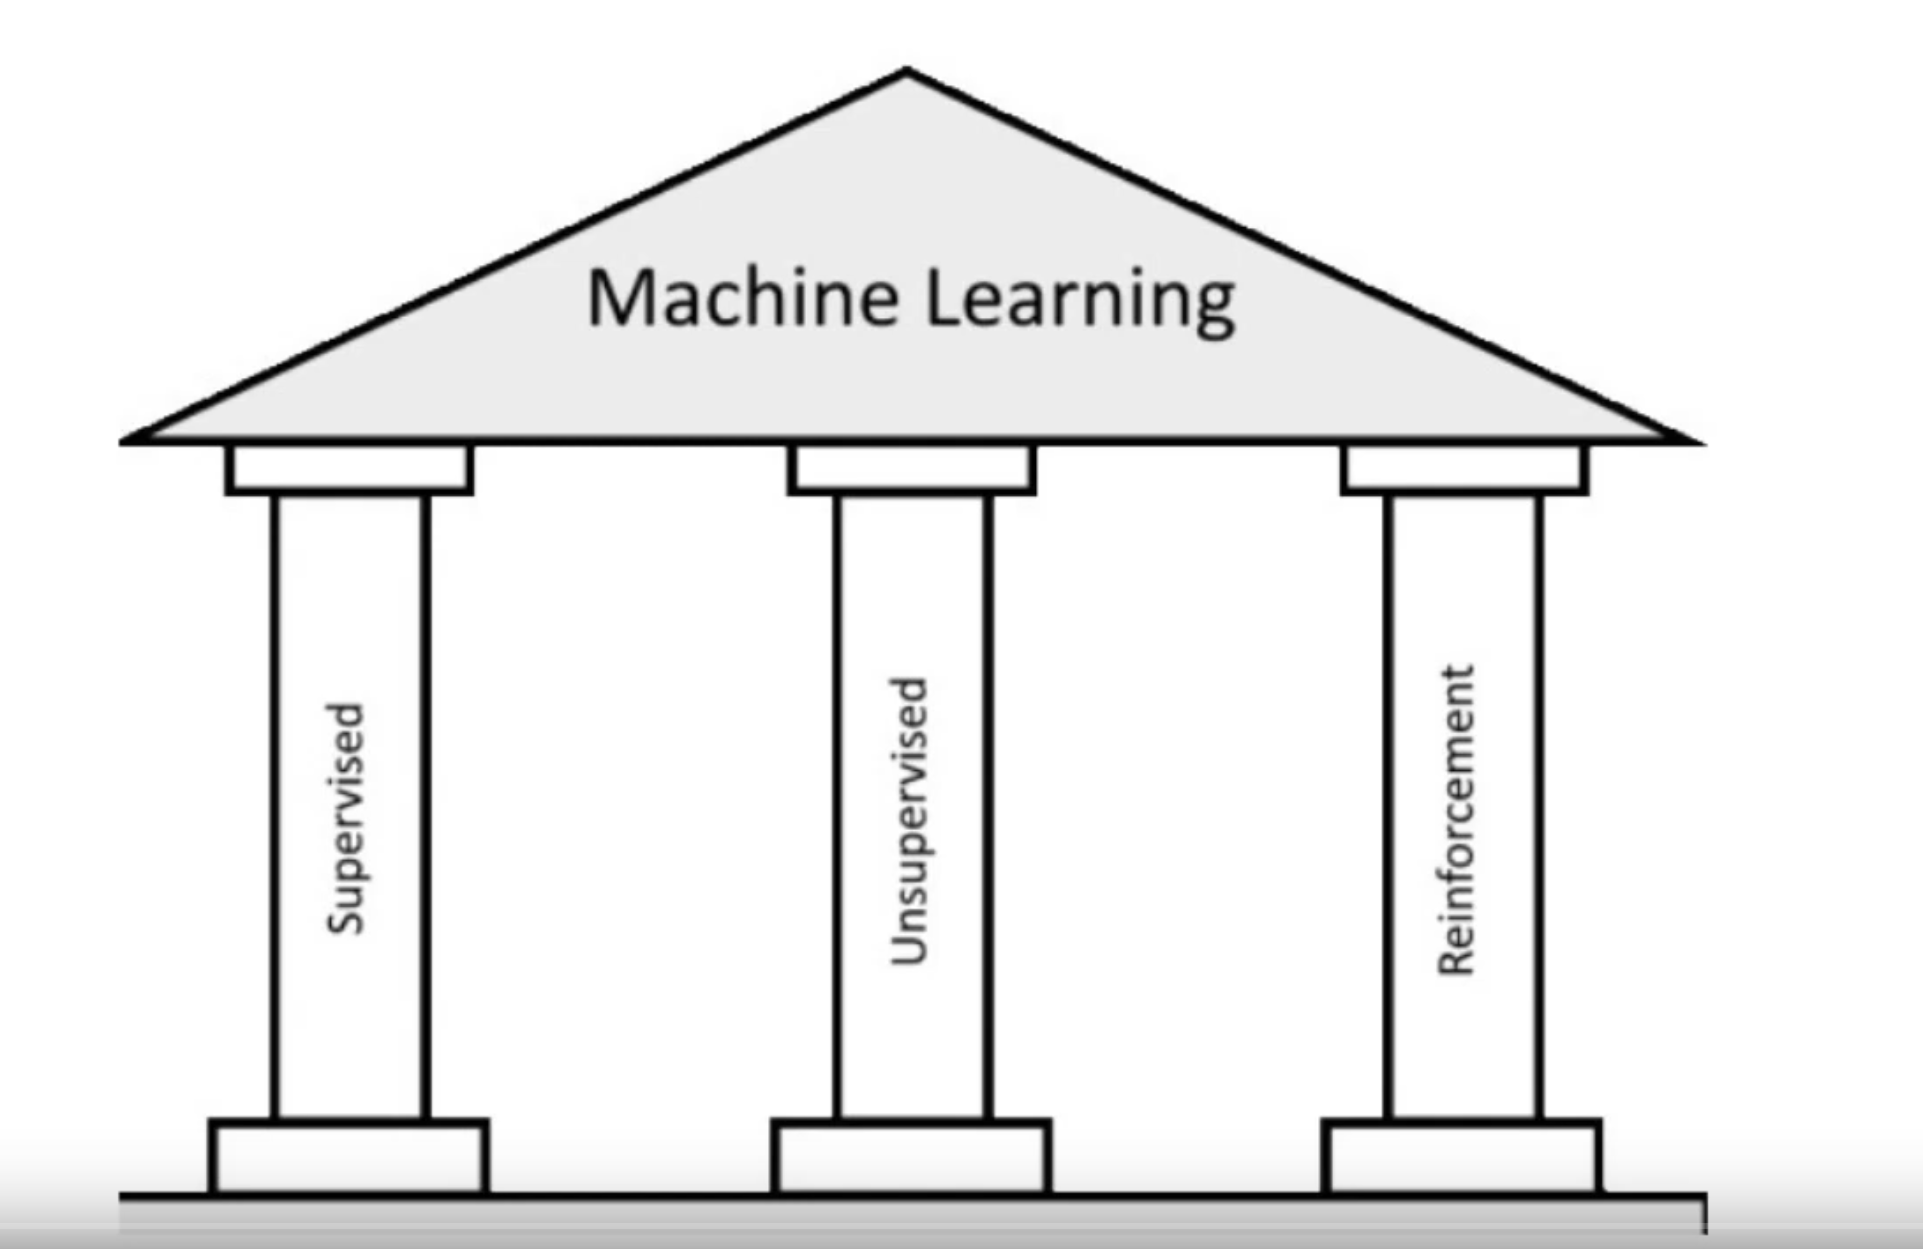
\includegraphics[width=0.6\linewidth]{machine.png}
  \end{figure}
  
\end{frame}
%------------------------------------------------

\begin{frame}
  \frametitle{¿Qué es el aprendizaje?}

  Norbert Wiener en su libro "Dios y el Golem" define aprendizaje como:
  
  \begin{definition}
    Un sistema organizado puede definirse como aquel que transforma un cierto mensaje de entrada en uno de salida, de acuerdo con algún principio de transformación. Si tal principio está sujeto a cierto criterio de validez de funcionamiento, y si el método de transformación se ajusta a fin de que tienda a mejorar el funcionamiento del sistema de acuerdo con ese criterio, se dice que el sistema aprende"
  \end{definition}

  \begin{figure}
    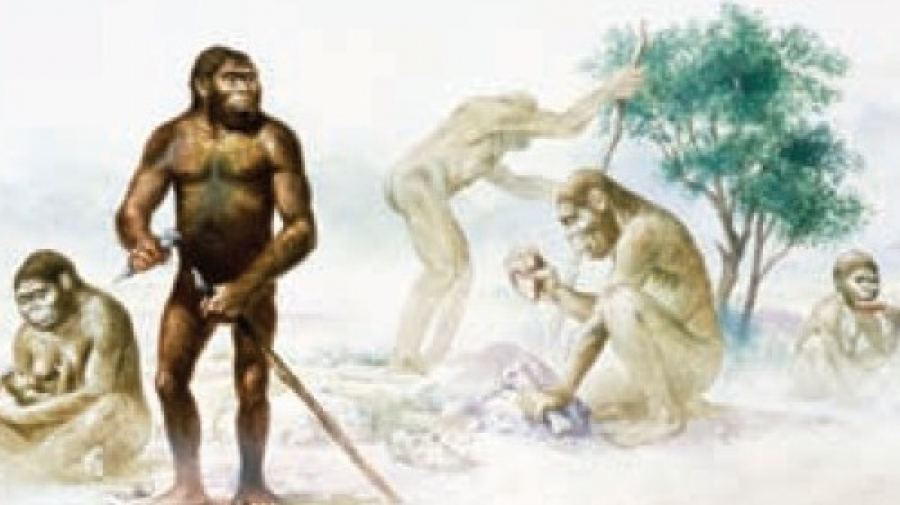
\includegraphics[width=0.4\linewidth]{homo.jpg}
  \end{figure}
  
\end{frame}


\subsection{Aprendizaje supervisado}
\begin{frame}
  \frametitle{Aprendizaje supervisado}

  Surge en enseñarle a estos algoritmos cual es el resultado que quieres obtener para un determinado valor tras mostrarles muchos ejemplos si se dan las condiciones, el algoritmo será capaz de dar un resultado correcto incluso cuando le muestres valores que no ha visto antes.

  \smallskip % Vertical whitespace

  Se denomina "clasificación"

  \begin{itemize}
    \item Los datos deben estar etiquetados, requiere supervisión humana.
    \item Se usan datos etiquetados para entrenamiento y se predicen individuos fuera de la muestra de entrenamiento
  \end{itemize}
  
  \smallskip % Vertical whitespace

  A partir de nuestros datos etiquetados entrenar un algoritmo que aprenda en relación a sus atributos.
    
\end{frame}

%------------------------------------------------
\subsection{Aprendizaje no supervisado ó "clustering"}
\begin{frame}
  \frametitle{Aprendizaje no supervisado}

  \begin{figure}
    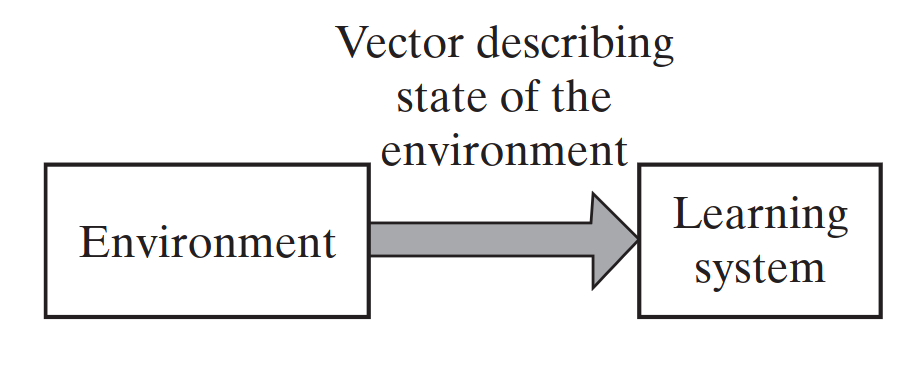
\includegraphics[width=0.4\linewidth]{unsupervised.png}
  \end{figure}
  
  No existe alguien que enseñe o evalue el proceso de aprendizaje, la red desarrolla la habilidad de formar representaciones internas para abstraer caracteristicas de la entrada y crear nuevas clases automaticamente.

  \bigskip % Vertical whitespace
  
  \begin{itemize}
    \item Los datos no están etiquetados
    \item El algortitmo busca por su cuenta grupos o cluster
  \end{itemize}

  \bigskip % Vertical whitespace
  
  Nuestro algoritmo es ciego y sólo conoce los atributos y en base a esas caracteristicas crear grupos

\end{frame}

\begin{frame}

  Se hace uso de reglas de aprendizaje competitivas "winner-takes-all"

  \bigskip % Vertical whitespace

  \begin{itemize}
     \item Capa de entrada recibe la información disponible 
     \item Capa competitiba consiste de neuronas que compiten entre ellas (en base a la regal de aprendizaje) para la esperanza de responder, la neurona con el mejor acierto ganara y se activará, dejando a las demas neuronas apagadas.
  \end{itemize}
  
\end{frame}

\subsection{Aprendizaje por refuerzo}
\begin{frame}
  \frametitle{Aprendizaje por refuerzo ¿Fuerza Bruta?}
  
  No tenemos una "etiqueta de salida", por lo que no es de tipo supervisado y si bien estos algoritmos aprenden por sí mismos, tampoco son de tipo no supervisado, en donde se intenta clasificar grupos teniendo en cuenta alguna distancia entre muestras.

  \bigskip % Vertical whitespace

  El Aprendizaje por refuerzo, intentará hacer aprender a la máquina basándose en un esquema de "premios y castigos" - en un entorno en donde hay que tomar acciones y que está afectando por múltiples variables que cambian con el tiempo.

  \bigskip % Vertical whitespace

  En modelos de Aprendizaje Supervisado (o no supervisado) se intenta minimizar la función de coste,.. es decir reducir el error.

  \bigskip % Vertical whitespace

  En cambio en Aprendizaje Reforzado intenta "maximizar la recompensa" con la continua interacción con el ambiente para minimizar el index scalar de desempeño.

\end{frame}

\begin{frame}
  \frametitle{Componentes del RL}

  \begin{figure}
    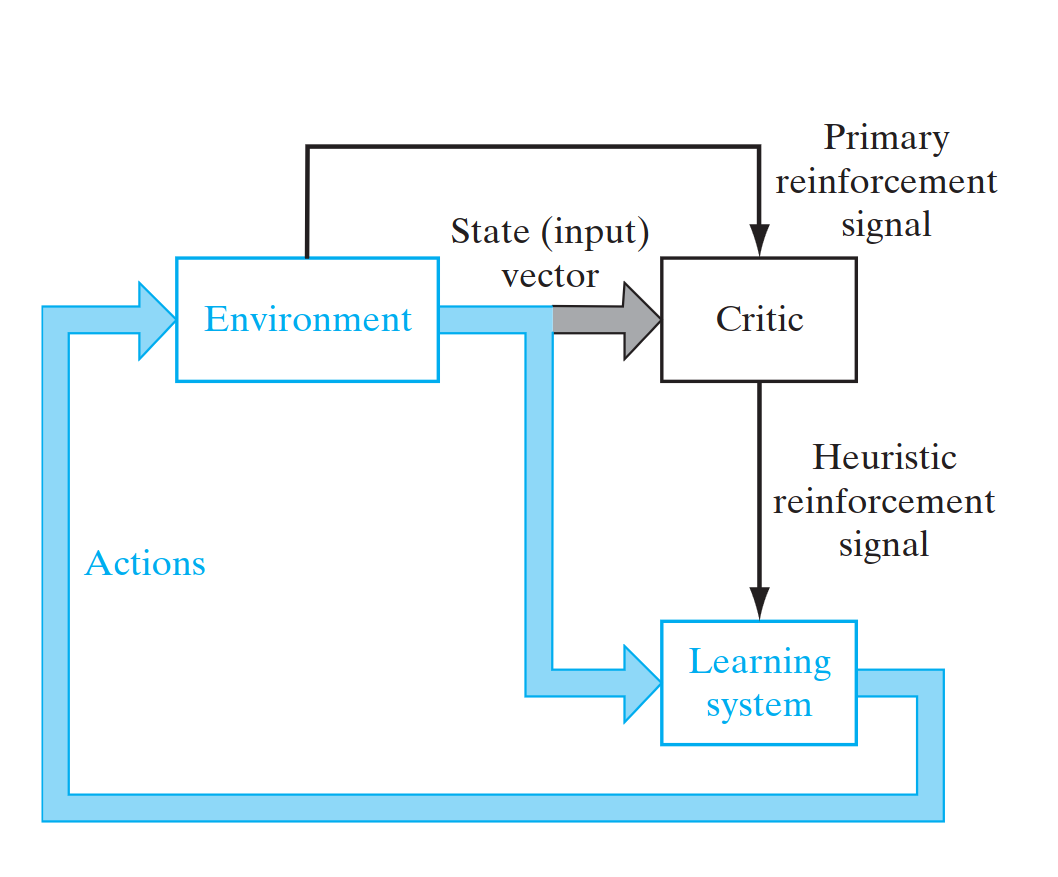
\includegraphics[width=0.3\linewidth]{RL.png}
  \end{figure}
  
  \begin{itemize}
  \item Agente - será nuestro modelo que queremos entrenar y que aprenda a tomar decisiones
  \item Ambiente - será el entorno en donde interactúa y se mueve el agente. Contiene las limitaciones y reglas posibles en cada momento
  \item Acción - posibles acciones que puede tomar en un momento determinado el agente
  \item Recompensas (ó castigos) - podremos obtener un premio ó penalización que oriente al agente en si lo está haciendo bien o mal.
  \end{itemize}

  \bigskip % Vertical whitespace
  
  Si la recompensa es positiva estaremos \alert{reforzando} ese comportamiento para el futuro. En cambio si la recompensa es negativa lo estaremos penalizando, para que ante la misma sutuación el agente actúe de manera distinta. 
  
\end{frame}

\begin{frame}
  \frametitle{Q-Learning, el algoritmo más usado}

  El objetivo es entrenar nuestro modelo a través de simulaciones de manera que las decisiones que vaya toamdno nuestro agente obtengan "la mayor recompensa"
  
  \begin{itemize}
  \item Politicas - Tabla que indicará al modelo como actuar en cada estado
  \item Acciones - las diversas acciones que puede hacer el agente
  \item Recompensas - si sumamos ó restamos puntaje con la acción tomada
  \item Comportamiento greedy - Tener grandes recompensas inmediatas o ir explorando y valorando las riquezas a largo plazo
  \end{itemize}

  
\end{frame}
%------------------------------------------------


\end{document} 
